\renewcommand{\arraystretch}{1.5} % Adjust the row height
\setlength{\tabcolsep}{0pt} % Remove extra padding between columns
\begin{center}
\resizebox{\textwidth}{!}{%
    \(
    \begin{array}{|p{0.4cm}|p{0.4cm}|p{0.4cm}|p{0.4cm}|}
    \hline
     &  &  &  \\ \hline
    \( \mathcal{\( A^* \)} \) &  & \( \mathcal{\( A^* \)} \) & \( \mathcal{\( A^* \)} \) \\ \hline
    \( \mathcal{\( A^* \)} \) & \( \mathcal{\( A^* \)} \) &  & \( \mathcal{\( A^* \)} \) \\ \hline
    \( \mathcal{\( A^* \)} \) & \( \mathcal{\( A^* \)} \) & \( \mathcal{\( A^* \)} \) &  \\ \hline
    \end{array}
    \hspace{2pt} % Decrease space here
    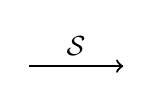
\begin{tikzpicture}[baseline={(current bounding box.center)}, scale=0.4]
        % Arrow from first grid to second grid
        \draw[->, thick] (0, 0) -- (3, 0)
            node[midway, above] {\( \mathcal{S} \)};
    \end{tikzpicture}
    \hspace{2pt} % Decrease space here
    \begin{array}{|p{0.4cm}|p{0.4cm}|p{0.4cm}|p{0.4cm}|}
    \hline
     &  &  &  \\ \hline
    \( \mathcal{\( A^* \)} \) &  & \( \mathcal{\( A^* \)} \) & \( \mathcal{\( A^* \)} \) \\ \hline
    \( \mathcal{\( A^* \)} \) & \( \mathcal{\( A^* \)} \) &  & \( \mathcal{\( A^* \)} \) \\ \hline
    \( \mathcal{\( A^* \)} \) & \( \mathcal{\( A^* \)} \) & \( \mathcal{\( A^* \)} \) &  \\ \hline
    \end{array}
    \hspace{2pt} % Decrease space here
    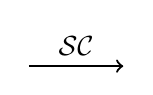
\begin{tikzpicture}[baseline={(current bounding box.center)}, scale=0.4]
        % Arrow from second grid to third grid
        \draw[->, thick] (0, 0) -- (3, 0)
            node[midway, above] {\( \mathcal{SC} \)};
    \end{tikzpicture}
    \hspace{2pt} % Decrease space here
    \begin{array}{|p{0.4cm}|p{0.4cm}|p{0.4cm}|p{0.4cm}|}
    \hline
     & \( \mathcal{\( A^* \)} \) & \( \mathcal{\( A^* \)} \) & \( \mathcal{\( A^* \)} \) \\ \hline
     &  & \( \mathcal{\( A^* \)} \) & \( \mathcal{\( A^* \)} \) \\ \hline
     & \( \mathcal{\( A^* \)} \) &  & \( \mathcal{\( A^* \)} \) \\ \hline
     & \( \mathcal{\( A^* \)} \) & \( \mathcal{\( A^* \)} \) &  \\ \hline
    \end{array}
    \hspace{2pt} % Decrease space here
    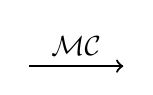
\begin{tikzpicture}[baseline={(current bounding box.center)}, scale=0.4]
        % Arrow from third grid to fourth grid
        \draw[->, thick] (0, 0) -- (3, 0)
            node[midway, above] {\( \mathcal{MC} \)};
    \end{tikzpicture}
    \hspace{2pt} % Decrease space here
    \begin{array}{|p{0.4cm}|p{0.4cm}|p{0.4cm}|p{0.5cm}|}
    \hline
     &  &  &  \\ \hline
     & \( \mathcal{A$_{2}$} \) &  &  \\ \hline
     &  & \( \mathcal{A$_{1}$} \) &  \\ \hline
     &  &  & \( \mathcal{A$_{3}$} \) \\ \hline
    \end{array}
    \hspace{2pt} % Decrease space here

    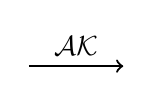
\begin{tikzpicture}[baseline={(current bounding box.center)}, scale=0.4]
        % Arrow from third grid to fourth grid
        \draw[->, thick] (0, 0) -- (3, 0)
            node[midway, above] {\( \mathcal{AK} \)};
    \end{tikzpicture}
    \hspace{2pt} % Decrease space here
    \begin{array}{|p{0.4cm}|p{0.4cm}|p{0.4cm}|p{0.5cm}|}
    \hline
     &  &  &  \\ \hline
     & \( \mathcal{A$_{2}$} \) &  &  \\ \hline
     &  &\( \mathcal{A$_{1}$} \) &  \\ \hline
     &  &  & \( \mathcal{A$_{3}$} \) \\ \hline
    \end{array}
    
}
\end{center}
\vspace{15}
\resizebox{\textwidth}{!}{%
    \(
    % \begin{array}{|p{0.4cm}|p{0.4cm}|p{0.4cm}|p{0.4cm}|}
    % \hline
    % \( \mathcal{A} \) &  &  &  \\ \hline
    %  &  &  &  \\ \hline
    %  &  &  &  \\ \hline
    %  &  &  &  \\ \hline
    % \end{array}
    \hspace{2pt} % Decrease space here
    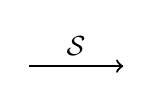
\begin{tikzpicture}[baseline={(current bounding box.center)}, scale=0.4]
        % Arrow from first grid to second grid
        \draw[->, thick] (0, 0) -- (3, 0)
            node[midway, above] {\( \mathcal{S} \)};
    \end{tikzpicture}
    \hspace{2pt} % Decrease space here
    \begin{array}{|p{0.4cm}|p{0.4cm}|p{0.4cm}|p{0.5cm}|}
    \hline
     &  &  &  \\ \hline
     & A$_{2}$ &  &  \\ \hline
     &  & A$_{1}$ &  \\ \hline
     &  &  & A$_{3}$ \\ \hline
    \end{array}
    \hspace{2pt} % Decrease space here
    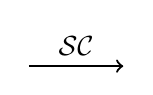
\begin{tikzpicture}[baseline={(current bounding box.center)}, scale=0.4]
        % Arrow from second grid to third grid
        \draw[->, thick] (0, 0) -- (3, 0)
            node[midway, above] {\( \mathcal{SC} \)};
    \end{tikzpicture}
    \hspace{2pt} % Decrease space here
    \begin{array}{|p{0.4cm}|p{0.4cm}|p{0.4cm}|p{0.4cm}|}
    \hline
     &  &  &  \\ \hline
    \( \mathcal{A$_{1}$} \) &  &  &  \\ \hline
    \( \mathcal{A$_{2}$} \) &  &  &  \\ \hline
    \( \mathcal{A$_{3}$} \) &  &  &  \\ \hline
    \end{array}
    \hspace{2pt} % Decrease space here
    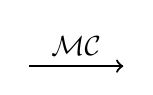
\begin{tikzpicture}[baseline={(current bounding box.center)}, scale=0.4]
        % Arrow from third grid to fourth grid
        \draw[->, thick] (0, 0) -- (3, 0)
            node[midway, above] {\( \mathcal{MC} \)};
    \end{tikzpicture}
    \hspace{2pt} % Decrease space here
    \begin{array}{|p{0.4cm}|p{0.4cm}|p{0.4cm}|p{0.4cm}|}
    \hline
     \( \mathcal{A} \) &  &  &  \\ \hline
     &  &  &  \\ \hline
     &  &  &  \\ \hline
     &  &  & \\ \hline
    \end{array}
    \)
    \hspace{2pt} % Decrease space here

    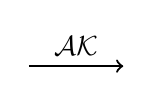
\begin{tikzpicture}[baseline={(current bounding box.center)}, scale=0.4]
        % Arrow from third grid to fourth grid
        \draw[->, thick] (0, 0) -- (3, 0)
            node[midway, above] {\( \mathcal{AK} \)};
    \end{tikzpicture}
    \hspace{2pt} % Decrease space here
   
    \begin{array}{|p{0.4cm}|p{0.4cm}|p{0.4cm}|p{0.4cm}|}
    \hline
     \( \mathcal{A} \) &  &  &  \\ \hline
     & &  &  \\ \hline
     &  &   &  \\ \hline
     &  &  &  \\ \hline
    \end{array}
    \)
    
}

\hspace{2pt} % Decrease space here

\[
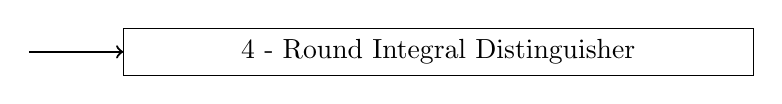
\begin{tikzpicture}[baseline={(current bounding box.center)}, scale=0.4]
    % Arrow from left to the box
    \draw[->, thick] (0, 0) -- (3, 0)
        node[midway, above] {};
    % Add the box at the end of the arrow
    \draw (3, -0.75) rectangle ++(20, 1.5) node[pos=.5] {4 - Round Integral Distinguisher};
\end{tikzpicture}
\]

\end{center}
